Im Folgenden wird die Hardware für die Programmierschnittstellen beschrieben. Es ist darauf zu achten, dass in Abbildung \ref{fig:Schema_USB_B} nur das Schema für die Programmierschnittstelle des WiFi-Moduls zu sehen ist. Vorab: Bei den Leitungen DTR, DSR, RTC, CTS, RXD und TXD handelt es sich um die Kommunikationsleitungen zwischen dem USB-UART-Konverter und dem Target. In Tabelle \ref{tab:USB_ESP} sind die Unterschiede tabellarisch aufgelistet.

\begin{table}[H]
\center
\begin{tabular}{|c|lcl|c||l|}
\hline
\textbf{Leitung} & & & & \textbf{Konverter} & \textbf{Target} \\ \hline
RXD & <== & über Widerstand & === & TX & beide \\
TXD & === & über WIderstand & ==> & RX & beide\\
IO\_0 / Reset & <== & über Transistor & === & DTR & beide\\
EN & <== & über Transistor & === & RTS & nur WiFi-Modul\\
IO\_13 & <== & über Widerstand & === & RTS & nur WiFi-Modul\\
IO\_15 & <== & über Widerstand & === & CTS & nur WiFi-Modul\\
\hline
\end{tabular}
\caption{Verbindung zwischen USB und WiFi-Modul.}
\label{tab:USB_ESP}
\end{table}

\paragraph{Schema}\mbox{}

Das USB-Kabel wird an der Buchse J2 angeschlossen. Sobald ein USB-Kabel eingesteckt ist, sind die Leiterplatine und der Computer auf gleichem Ground-Potential und die Leitungen D+ und D- mit dem Konverter verbunden. Über das USB-Kabel werden ebenfalls 5V am Spannungsteiler R12 und R13 angelegt, was vom Konverter als bestehende USB-Verbindung interpretiert wird. Da beim Einstecken die Gefahr von Spannungsdifferenzen besteht, wird ein ESD-Schutz benötigt, welcher vom den Dioden D2-4 gewährleistet wird. Die LED's können verwendet werden, um einen Datenfluss zu signalisieren. Die Widerstände in den Kommunikations- und Steuerleitungen schützen die Pins vor hohen Strömen im Falle von Spannungsunterschieden.
\begin{figure}[h!]
	\centering
	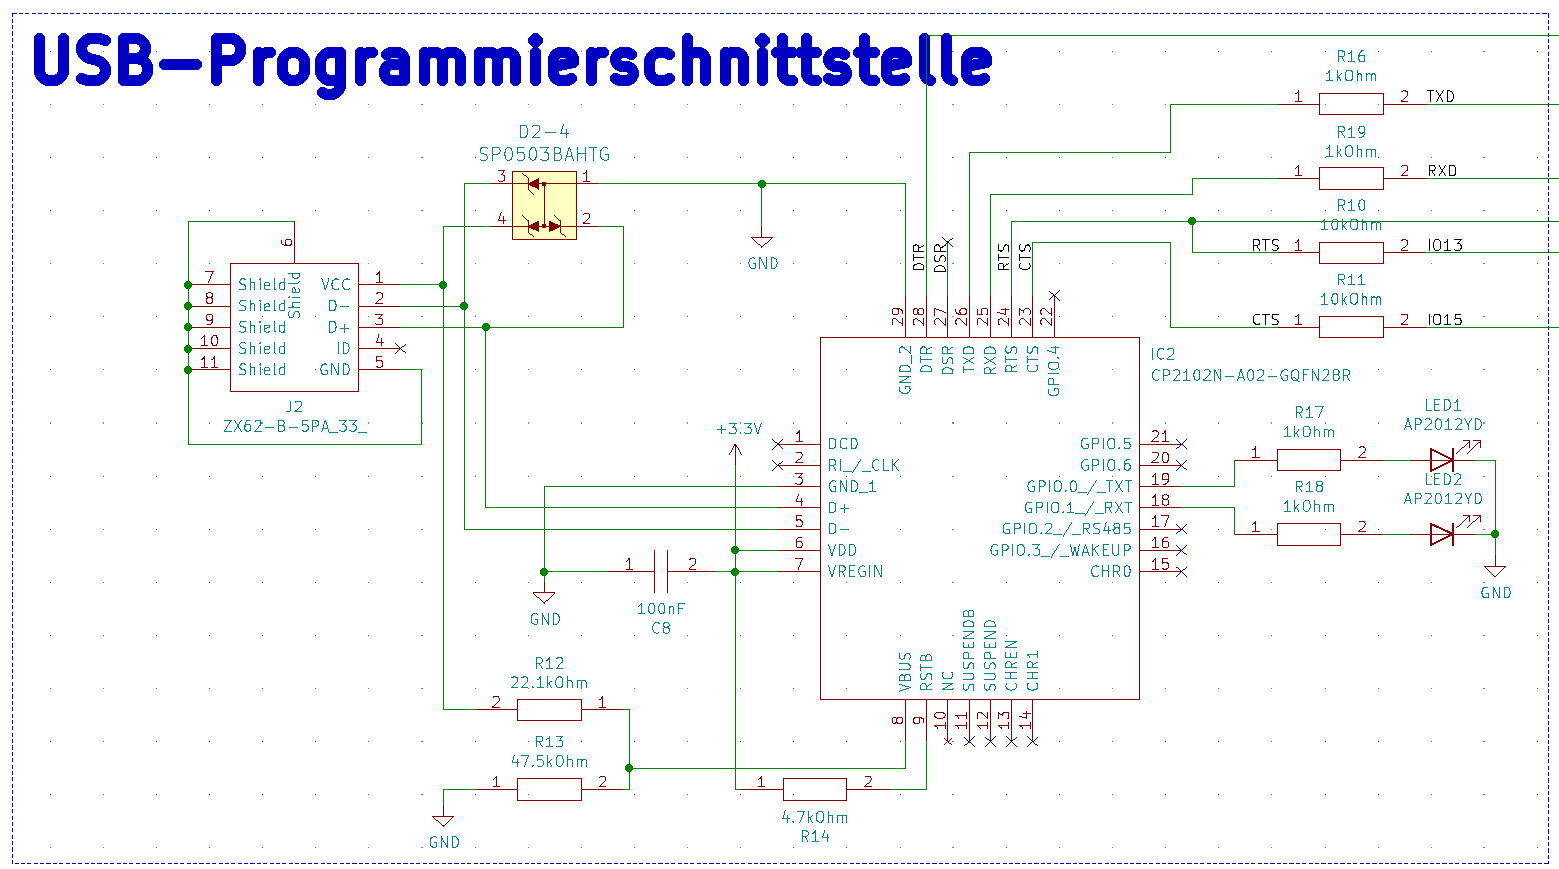
\includegraphics[width=1\textwidth]{graphics/Schema_USB_B}
	\caption{Schema USB-B.}
	\label{fig:Schema_USB_B}
\end{figure}
\newpage
\paragraph{Funktionsbeschrieb der Schaltung}\mbox{}

Der dazugehörige ESD-Schutz bildet die Diodenschaltung D2-D4. Dabei handelt es sich um ESD-Schutzdioden des Typs SP0503BAHTG. Sie werden ab einer Spannung von 3.3V leitend und reduzieren so die maximale Spannung auf den Eingangspins des Konverters auf 3.3V. Der Konverter hat im Schema die Bezeichnung IC2. Es ist ein CP2102N des Herstellers Silicon-Labs. Die Widerstände R12 und R13 bilden einen Spannungsteiler, welcher an die 5V-Eingangsspannung der Buchse und an dem VBUS-Eingang des Converters hängt. Die Widerstände R16, R19, R10 und R11 reduzieren die Ausgleichsströme zwischen dem USB-UART-Converter und dem Target (WiFi-Modul oder Mikrocontroller). Der Widerstand R14 ist ein Pull-Up Widerstand, welcher verhindert, dass der Reset-Pin des Konverters einen ungewünschten Zustand annimmt. Die Widerstände R17 und R18 reduzieren den Strom durch die LED's.